\documentclass[12pt,fleqn,answers]{exam}
\usepackage{pifont}
\usepackage{dingbat}
\usepackage{amsmath,amssymb}
\usepackage{epsfig}
\usepackage[colorlinks=true,linkcolor=black,anchorcolor=black,citecolor=black,filecolor=black,menucolor=black,runcolor=black,urlcolor=black]{hyperref}
\usepackage[letterpaper, margin=0.75in]{geometry}
\addpoints
\boxedpoints
\pointsinmargin
\pointname{pts}

\usepackage[final]{microtype}
\usepackage[american]{babel}
%\usepackage[T1]{fontenc}
\usepackage{fourier}
\usepackage{isomath}
\usepackage{upgreek,amsmath}
\usepackage{amssymb}

\newcommand{\dotprod}{\, {\scriptzcriptztyle
    \stackrel{\bullet}{{}}}\,}

\newcommand{\reals}{\mathbf{R}}
\newcommand{\lub}{\mathrm{lub}} 
\newcommand{\glb}{\mathrm{glb}} 
\newcommand{\complex}{\mathbf{C}}
\newcommand{\dom}{\mbox{dom}}
\newcommand{\range}{\mbox{range}}
\newcommand{\cover}{{\mathcal C}}
\newcommand{\integers}{\mathbf{Z}}
\newcommand{\vi}{\, \mathbf{i}}
\newcommand{\vj}{\, \mathbf{j}}
\newcommand{\vk}{\, \mathbf{k}}
\newcommand{\bi}{\, \mathbf{i}}
\newcommand{\bj}{\, \mathbf{j}}
\newcommand{\bk}{\, \mathbf{k}}
\newcommand{\dist}{\, \mathrm{dist}}
\DeclareMathOperator{\Arg}{\mathrm{Arg}}
\DeclareMathOperator{\Ln}{\mathrm{Ln}}
\newcommand{\imag}{\, \mathrm{i}}

\usepackage{xcolor}
\shadedsolutions
\definecolor{SolutionColor}{rgb}{0.95,0.95,0.95}

\usepackage{graphicx}
\newcommand\AM{{\sc am}}
\newcommand\PM{{\sc pm}}
     
\usepackage{twemojis}
\newcommand{\quiz}{2}
\newcommand{\term}{Spring}
\newcommand{\due}{9:55 \AM}
\newcommand{\class}{MATH 102}
\begin{document}
\large
\vspace{0.1in}
\noindent\makebox[3.0truein][l]{\textbf{\class, \term \/ \the\year}}
\textbf{Name:} \hrulefill \\
\noindent \makebox[3.0truein][l]{\textbf{In class work \quiz}}
\textbf{Row and Seat}:\hrulefill\\
\vspace{0.1in}


\noindent  In class work  \quiz\/  has questions 1 through  \numquestions \/ with a total of  \numpoints\/  points.   
 This assignment is due at the end of the class period (\due).

\vspace{0.1in}


\begin{questions} 

\question A line $L$ contains the points $(x=5,y=2)$ and
$(x=7,y=-1)$.  

\begin{parts}

    \part [1] Find an \emph{equation} of the line $L$.
    \begin{solution}[1.5in] The slope of the line $L$ is
        \begin{equation*}
            \frac{2-(-1)}{5-7} = -\frac{3}{2}
        \end{equation*}    
        An equation of the line $L$ is
        \begin{equation*}
            y-2 = -\frac{3}{2} (x-5).
        \end{equation*}
        Using the other point, we get a syntactically different
        equation--it is
        \begin{equation*}
            y+1 = -\frac{3}{2} (x-7).
        \end{equation*}
        A good way to check an equation of a line is to paste
        the data in to the equation and see if it is true. Pasting
        $(x=5,y=2)$ into our first equation for $L$, we have
        \begin{equation*}
            \left[2-2 = -\frac{3}{2} (5-5) \right] = 
               \left[0 = 0\right] = \mbox{True}.
        \end{equation*}
        And pasting in $(x=7,y=-1)$, we have
        \begin{equation*}
            \left[-1-2 = -\frac{3}{2} (7-5) \right] = 
               \left[-3 = -3 \right] = \mbox{True}.
        \end{equation*}
        Similarly, you should check that the equation 
        $ y+1 = -\frac{3}{2} (x-7)$ is also correct.

        The question \emph{doesn't} ask for a particular form for 
        the equation of the line, but converting to a slope-intercept 
        form, we have
        \begin{equation*}
            y = -\frac{3}{2}  x + \frac{19}{2}.
        \end{equation*} 

    \end{solution}

    \part  [1] Find the \emph{x-intercept} of the line $L$.
    \begin{solution}[1.5in] To find the x-intercept of the line
        $y-2 = -\frac{3}{2} (x-5)$, set $y$ to zero and solve for $x$; we have
        \begin{align*}
            \left[0-2 = -\frac{3}{2} (x-5) \right] &= \left[\frac{4}{3}  = x-5 \right], \\
                       &= \left[x = \frac{19}{3} \right]
        \end{align*}


    \end{solution}

    \part [1] Find the \emph{y-intercept} of the line $L$.
    \begin{solution}[1.5in] To find the y-intercept of the line
        $y-2 = -\frac{3}{2} (x-5)$, set $x$ to zero and solve for $y$; we have
        \begin{align*}
            \left[y-2 = -\frac{3}{2} (0-5) \right] &= 
                \left[ y-2 = \frac{15}{2} \right] \\
                &= \left[ y = \frac{19}{2} \right] \\
        \end{align*}
    \end{solution}
\end{parts}

\newpage

\question An equation of a line $L$ is $2 y + 3 x = 6$.

\begin{parts}

    \part [1] Find the \emph{slope} of the line $L$.
    \begin{solution}[1.5in] To find the slope of the line $2 y + 3 x = 6$,
        we solve $2 y + 3 x = 6$ for $y$ and match to the slope-intercept form
        $y= mx + b$ (the slope being $m$). Solving $2 y + 3 x = 6$ for
        $y$ gives $y = -\frac{3}{2} x + 3$. And matching this to $y= mx + b$ gives
        $m = -\frac{3}{2}$.

    \end{solution}
   
    \part [1] Find the \emph{x-intercept} of the line $L$.
    \begin{solution}[1.5in] We have
        \begin{equation*}
            \left[3 x = 6\right] = \left[x = 2 \right].
        \end{equation*}
    \end{solution}

    \part [1] Find the \emph{y-intercept} of the line $L$.
    \begin{solution}[1.5in] We have
        \begin{equation*}
            \left[2 y = 6\right] = \left[ y = 3 \right].
        \end{equation*}
    \end{solution}


    \part [1] Draw a graph of the line $L$.
    \begin{solution}[1.5in]
        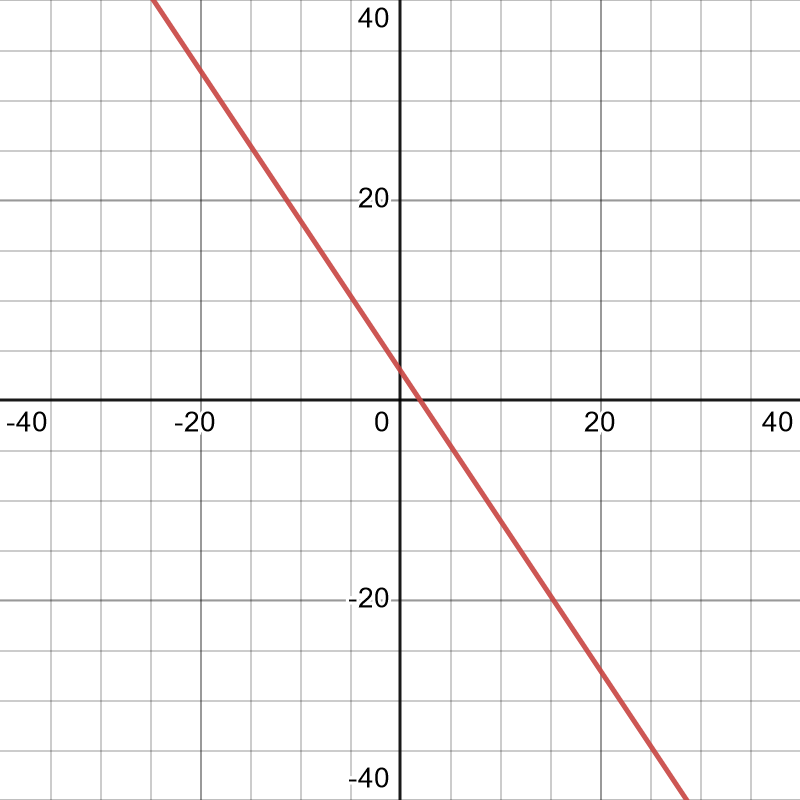
\includegraphics[scale=0.2]{desmos-graph(39).png}
    \end{solution}

\end{parts}
%
%\vfill 
%\newpage

%\question [2] Find an \emph{equation} of the line that is perpendicular 
%to the line $2 y + 3 x = 6$ and that contains the point $(x=6,y=6)$.

\end{questions}
\end{document}